\documentclass[11pt]{article}
\usepackage{fullpage}
\usepackage{setspace}
\usepackage{amsmath}
\usepackage{fancyvrb}
\usepackage{enumerate}
\usepackage{pgfplots}
\usepackage{graphicx}
\usepackage{float}

\begin{document}
\noindent\large{Math 5365}\\
\large{Data Mining 1}\\
\large{Homework 2}\\
\large{Mary Barker}
\newline

\begin{enumerate}
% 1
  \item Label the following as nominal, ordinal, or quantitative
    \begin{enumerate}
      \item Weight of content in a bag of chips. \textbf{Quantitative}
      \item City that a person lives in. \textbf{Nominal}
      \item Answers on a survey with set options for answers. \textbf{Ordinal}
    \end{enumerate}
% 2
  \item Give examples of the following two types of problems. 
    \begin{enumerate}
      \item Regression problems. \\
          Predicting the daily income for a caf\'{e} based on month of the year. 
          This is a regression problem because the dependent value(income) is 
          represented by numerical values that have mathematical significance. 
      \item Classification problems. \\
          Predicting customer orders based on season of the year. 
          This is a classification problem because what is being predicted 
          (which could be nominal or ordinal depending on how rigidly the 
          menu is adhered to) does not have meaningful numerical values. 
    \end{enumerate}
% 3
  \item The right hand limit $\lim \limits_{x \to 0^+}$ $x \log_2 x$ can be computed, since $\log_2 x$ is well defined for all $x > 0$. 
    In addition, entropy is defined as $- \sum \limits_{i = 0}^{c - 1} p_i \log_2 p_i$ where $p_i$ is the fraction of records 
    in class $i$. As a fraction that has maximum value of $\frac{c}{c}$, $p_i$ are always $0 \le p_i \le 1$. 
    In the components of the sum $- \sum \limits_{i = 0}^{c - 1} p_i \log_2 p_i$ the terms $\log_2 p_i$ are always less than or equal to 0. 
    Thus the entire sum is always greater than or equal to 0. 
    Now, since entropy is greater than or equal to 0, there is no definition for entropy less than zero, 
    and it is reasonable to define $x \log_2 x \left.\right|_{x = 0}$ as the limit 
    $\lim\limits_{x \to 0^+} x \log_2 x = 0$.  
% 4
  \item given the distribution $(p_0, p_1, ... , p_{c - 1})$, assume $p_j = 1$ and $p_i = 0 \forall i \neq j$. 
     \begin{enumerate}
       \item Entropy\\
         The formula for entropy is given by 
         $$- \sum \limits_{i = 0}^{c - 1} p_i \log_2 p_i$$ 
         Since all $p_i = 0$ for $i \ne j$, the terms $p_i \log_2 p_i$ reduce to 0 for all $i \ne j$. 
         The only element in this sum that contributes a potentially nonzero value is for $p_j$. 
         Now since $p_j = 1$, this term can be written $ p_j \log_2 p_j = 1\times\log_2(1) = 1 \times 0 = 0$. 
         Therefore every term in the sum is equal to 0, and the entire sum is equal to 0. 
       \item Gini\\
         The formula for Gini is given by 
         $$1 - \sum\limits_{i = 0}^{c - 1} p_i^2$$
         Now since $p_i = 0$ for all $i \ne j$, and $p_j = 1$, the sum 
         $$\sum\limits_{i = 0}^{c - 1} p_i^2$$ is equal to 
         $$\left(\sum\limits_{\substack{i = 0\\ i \ne j}}^{c - 1} 0^2\right) + 1^2$$
         which reduces to 1. 
         Therefore the total value for Gini is 
         $$ 1 - \sum\limits_{i = 0}^{c - 1} p_i^2 = 1 - 1 = 0$$
       \item Classification error\\
         The formula for classification error is 
         \\
         1 - max$_i$[$p_i$]
         \\
         Now, since all $p_i = 0, i \ne j$ and $p_j = 1$, the max$_i$[$p_i$] $= 1$. Therefore the classification factor is 
         $$1 - 1 = 0$$
      \end{enumerate}
%5
    \item Show mathematically that entropy, Gini and classification error impurity measures achieve maximum at $p_0 = p_1 = \frac{1}{2}$ 
          for a two class problem.\\
          Note that for a two class problem, $p_1 = 1 - p_0$. 
          \begin{enumerate}
            \item Gini\\
                 For the Gini measure, the formula is $$ 1 - \sum\limits_{j = 0}^{c - 1} p_j^2$$
                 Which is equal to $$1 - p_0^2 - (1 - p_0^2) = 1 - p_0^2 - 1 + 2p_0 - p_0^2$$
                 On the interval $[0, 1]$, the derivative of the function $$ f(x) = 2(x - x^2)$$
                 is equal to 0 when $2(1 - 2x) = 0$. That is, $x = \frac{1}{2}$. The only thing to check now is whether $f'(x)$ is 
                 positive on $[0, \frac{1}{2})$, and negative on $(\frac{1}{2}, 1]$. On $[0, \frac{1}{2}]$, the quantity $2x$ is always 
                 less than 1, and so $2(1 - 2x) > 0$. On $(\frac{1}{2}, 1]$, $2x > 1$, and so $2(1 - 2x) < 0$. Thus the maximum value 
                 is always achieved at $p_0 = \frac{1}{2}$, and $p_1 = 1 - p_0 = 1 - \frac{1}{2} = \frac{1}{2}$.
            \item entropy\\
                 The entropy measure is given by $$ -\sum\limits_{j = 0}^{c - 1} p_j \log_2 p_j$$
                 Since $p_1 = 1 - p_0$, the function that describes this is $f(x) =  - x \log_2(x) - (1 - x)\log_2(1 - x)$.
                 The derivative is 
                 \begin{equation}
                   \begin{array}{rl}
                      f'(x) = &-1\log_2(x) - \frac{x}{x\log(2)} - (-\log_2(1 - x)) + \frac{1 - x}{(1 - x) \log(2)}\\
                            = &-\log_2(x) - \frac{1}{\log(2)} + \log_2(1 - x) - \frac{1}{\log(2)}\\
                            = &-\log_2(x) - (-\log(2)) + \log_2(1 - x) - \log(2)\\
                            = &-\log_2(x) + \log_2(1 - x)\\
                   \end{array}
                 \end{equation}
                 This equation equals 0 when $(1 - x) = x$, so when $x = \frac{1}{2}$. As with the Gini measure, it is necessary to show 
                 that $f'(x) > 0$ $ \forall x \in [0, \frac{1}{2})$, and $f'(x) < 0$ $ \forall x \in (\frac{1}{2}, 1]$. 

                 Now, in $[0, \frac{1}{2})$, $x < 1 - x$. Therefore $\log_2(x) < \log_2(1 - x)$, and 
                 $\log_2(1 - x) - \log_2(x) > 0$.
                 In $(\frac{1}{2}, 1]$, $(1 - x) < x$, and therefore $\log_2(x) > \log_2(1 - x)$, and so $\log_2(1 - x) - \log_2(x) < 0$.
            \item Classification error\\
                 For this case, the formula is $$ 1 - max_j[p_j]$$ Now, the minimum value of $max_j[p_0, 1 - p_0]$, is $\frac{1}{2}$ for 
                 $p_0 \in [0, 1]$. 

          \end{enumerate}
%6
    \item Write a function in R that accepts a class distribution vector and returns the Gini impurity measure, and then 
          repeat for entropy and classification error measures. \\
          The functions are shown below. Test cases were run and verified by hand computations to show that they do indeed 
          perform the correct evaluations. 
\begin{Verbatim}[numbers=left]
# this program has a function that accepts a vector of arbitrary length and computes
# the Gini impurity, entropy and the classification error measures. 

# checks that the set of values does add up to 1.
# otherwise we're missing one or more sets.  
# this is a lazy code that just adds whatever is 
# needed to make it 1. 
check_add_to_1 = function(v1){
  value = sum(v1)
  if(value < 1){
  	v2 = rep(0, length(v1) + 1)
    v2 = c(v1, 1 - value)
  }
  if(value == 1){
  	v2 = v1
  }
  return(v2)
}

gini_eval = function(distribution_v){
  v = check_add_to_1(distribution_v)
  gini = 1 - sum(v * v)
  return(gini)
}

entropy_eval = function(distribution_v){
  # create a temporary array that has same entries as
  # distribution_v, except where distribution_v = 0. 
  # there tmp is 1 so I won't get nan computing 
  # log(tmp) (want the result to be 0 anyway)
  v = check_add_to_1(distribution_v)
  tmp = (v == 0) * 1
  tmp = tmp + v

  entropy = -1 * sum(tmp * (log(tmp) / log(2)))
  return(entropy)
}

class_error_eval = function(distribution_v){
  v = check_add_to_1(distribution_v)
  class_error = 1 - max(v)
  return(class_error)
}
\end{Verbatim}

%7
    \item Not a problem to be solved, an example of graphing a vector of values. 
%8
    \item Reproduce the plots of impurity measures on slide 17. 
      The code used to generate the plots is shown below. This segment was typed 
      into console while the script shown above was loaded. Each of the function 
      calls is therefore to a function shown in the code segment above. 
      The plots are color 
      coded where the Gini impurity measure is black, the entropy measure in green
      and the classification error in blue.
\begin{Verbatim}[numbers=left]
x = seq(from=0,to=1,by=0.01)
y1 <- rep(0, 101)
y2 <- rep(0, 101)
y3 <- rep(0, 101)
for(i in 1:100){
  y1[i] = gini_eval(x[i])
  y2[i] = entropy_eval(x[i])
  y3[i] = class_error_eval(x[i])
}
plot(x, y1, type='l',col='black', ylim=c(0,1))
lines(x, y2, type='l',col='green')
lines(x, y3, type='l',col='blue')
\end{Verbatim}

\begin{figure}[H]
\begin{center}
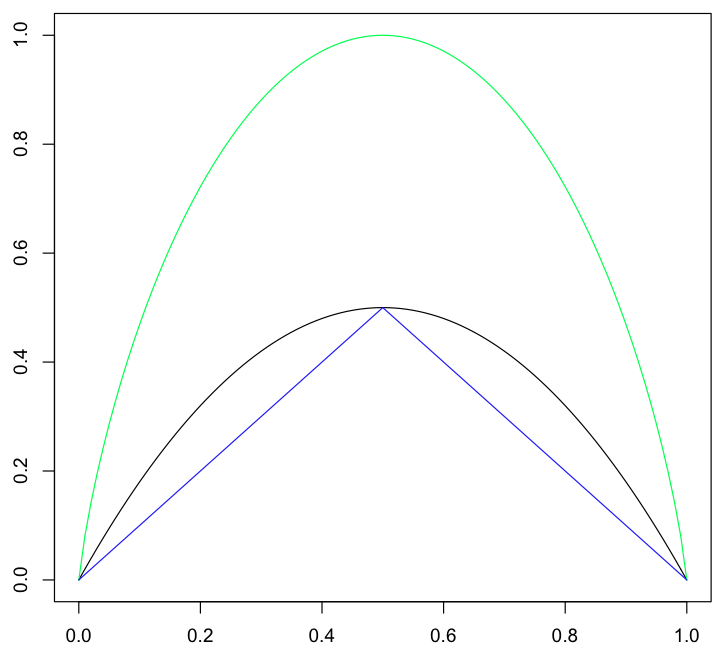
\includegraphics[scale=0.3]{graphsoferrormeasures}
\end{center}
\caption{graph of the impurity measures computed using the code listed}
\end{figure}

%9
    \item For this problem, the file Hw2.csv was loaded using a new script that 
also sourced the script measures.R that contains the function calls listed in 
Problem 6. There are 4 variables listed in this file. The values for each 
person are listed for gender, car type, shirt size and class label. 
The total number of people for whom these variables are recorded is 1000. 
\\
The code used to verify (a)-(b) is shown attached at the end. 
      \begin{enumerate}
        \item The values computed for this were N = 1000, C0 480, C1 520. 
        \item When splitting the data with respect to gender and then considering the 
              entropy of each branch with respect to class, the weighted entropy for 
              the node was computed as 0.9745739. The distribution is shown below. 
          \begin{figure}[H]
          \begin{center}
          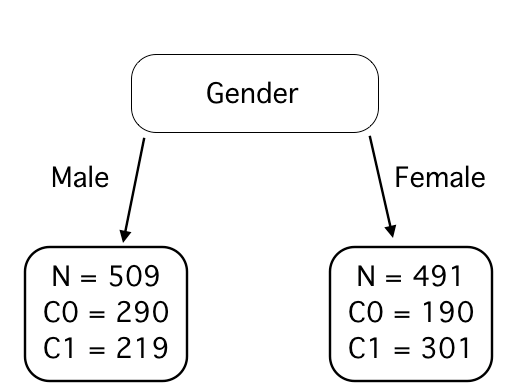
\includegraphics[scale=0.25]{genderclass}
          \end{center}
          \end{figure}
        \item The split for car type includes 3 different kinds: Family, Luxury, and Sports. 
              The weighted entropy for car type with respect to class is 0.3657676.
              The tree for this is shown below. 
          \begin{figure}[H]
          \begin{center}
          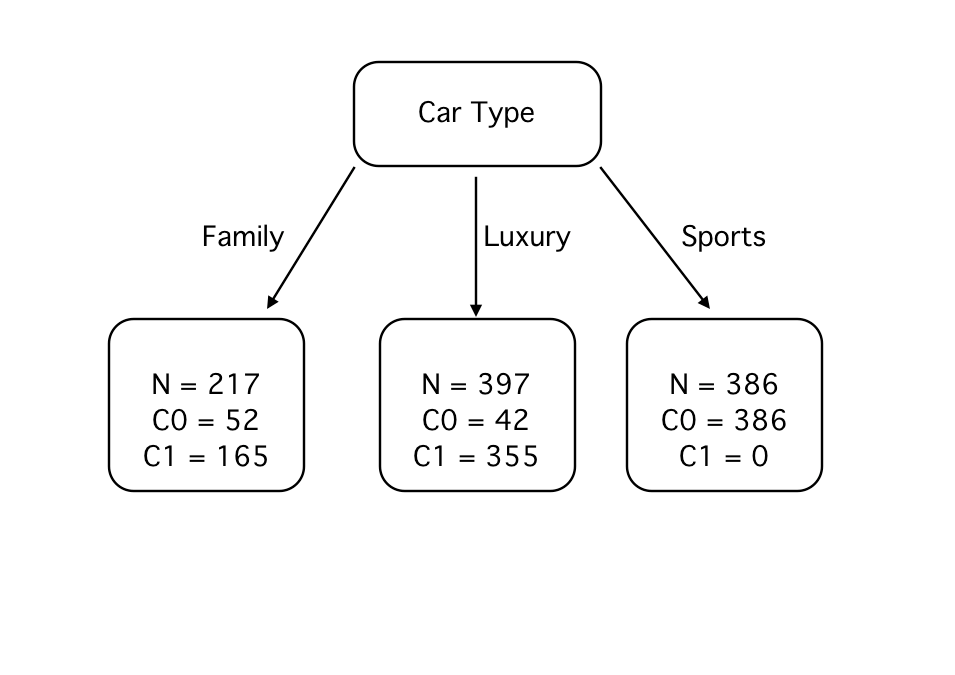
\includegraphics[scale=0.20]{cartypeclass}
          \end{center}
          \end{figure}
        \item For shirt size, there are 4 different possible choices: extra large, large, 
              medium and small. The weighted entropy for shirt size was 0.9771053. The 
              tree for this is shown below. 
          \begin{figure}[H]
          \begin{center}
          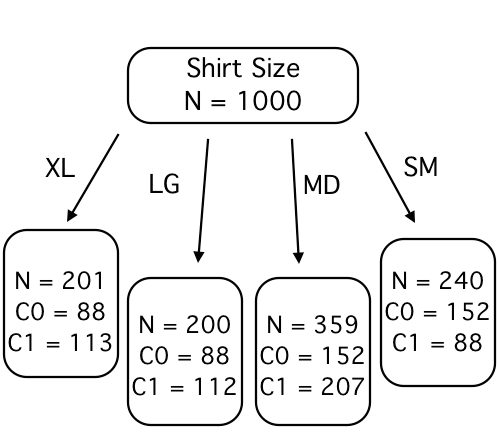
\includegraphics[scale=0.25]{shirtclass}
          \end{center}
          \end{figure}
        \item The minimum computed weighted entropy was for splittinng with respect to 
              car type first. Therefore this would be the best initial split. 
      \end{enumerate}
\end{enumerate}
\begin{Verbatim}[numbers=left]
people <- read.table("~/Dropbox/Tarleton/data_mining/hw02/Hw2.csv", 
                                                  header=TRUE, sep=",")

gender = people$Gender
cartype = people$CarType
shirtsize = people$ShirtSize
class = people$Class

N = length(class)
#typing 'N' into console now returns 1000

source("~/Dropbox/Tarleton/data_mining/hw02/measures.R")

#################################################
#             Test class entropy
#################################################
table(class)
#result of calling table(class) is the following: 
# C0   C1
#480  520
class1 = (class == 'C0')*1
class2 = (class == 'C1')*1
class_n1 = sum(class1)/N
class_n2 = sum(class2)/N
entropy = entropy_eval(c(class_n1, class_n2))
#typing 'entropy' into console results in 0.9988455 

#################################################
#         Test gender weighted entropy
#################################################
genderm = (gender == 'M')*1
genderf = (gender == 'F')*1

gender_n1 = sum(genderm)/N
gender_n2 = sum(genderf)/N

class11 = sum( ((genderm > 0) & (class1 > 0)) * 1)
class12 = sum( ((genderm > 0) & (class2 > 0)) * 1)
class21 = sum( ((genderf > 0) & (class1 > 0)) * 1)
class22 = sum( ((genderf > 0) & (class2 > 0)) * 1)

class11 = class11 / sum(genderm)
class12 = class12 / sum(genderm)
class21 = class21 / sum(genderf)
class22 = class22 / sum(genderf)

e1 = entropy_eval(c(class11, class12))
e2 = entropy_eval(c(class21, class22))
weighted_entropy = (gender_n1 * e1 + gender_n2 * e2) 

#################################################
#         Test cartype weighted entropy
#################################################
fam = (cartype == 'Family')*1
lux = (cartype == 'Luxury')*1
spt = (cartype == 'Sports')*1

car_n1 = sum(fam) / N
car_n2 = sum(lux) / N
car_n3 = sum(spt) / N

class11 = sum( (fam > 0) & (class1 > 0) )
class12 = sum( (fam > 0) & (class2 > 0) )
class21 = sum( (lux > 0) & (class1 > 0) )
class22 = sum( (lux > 0) & (class2 > 0) )
class31 = sum( (spt > 0) & (class1 > 0) )
class32 = sum( (spt > 0) & (class2 > 0) )

class11 = class11 / sum(fam)
class12 = class12 / sum(fam)
class21 = class21 / sum(lux)
class22 = class22 / sum(lux)
class31 = class31 / sum(spt)
class32 = class32 / sum(spt)

e1 = entropy_eval(c(class11, class12))
e2 = entropy_eval(c(class21, class22))
e3 = entropy_eval(c(class31, class32))

weighted_entropy = car_n1 * e1 + car_n2 * e2 + car_n3 * e3

#################################################
#         Test shirtsize weighted entropy
#################################################
table(shirtsize)
x = (shirtsize == 'ExtraLarge')*1 # 201
l = (shirtsize == 'Large')*1      # 200
m = (shirtsize == 'Medium')*1     # 359
s = (shirtsize == 'Small')*1      # 240
shirt_n1 = sum(x) / N
shirt_n2 = sum(l) / N
shirt_n3 = sum(m) / N
shirt_n4 = sum(s) / N

class11 = sum( (x > 0) & (class1 > 0) )
class12 = sum( (x > 0) & (class2 > 0) )
class21 = sum( (l > 0) & (class1 > 0) )
class22 = sum( (l > 0) & (class2 > 0) )
class31 = sum( (m > 0) & (class1 > 0) )
class32 = sum( (m > 0) & (class2 > 0) )
class41 = sum( (s > 0) & (class1 > 0) )
class42 = sum( (s > 0) & (class2 > 0) )

class11 = class11 / sum(x)
class12 = class12 / sum(x)
class21 = class21 / sum(l)
class22 = class22 / sum(l)
class31 = class31 / sum(m)
class32 = class32 / sum(m)
class41 = class41 / sum(s)
class42 = class42 / sum(s)

e1 = entropy_eval(c(class11, class12))
e2 = entropy_eval(c(class21, class22))
e3 = entropy_eval(c(class31, class32))
e4 = entropy_eval(c(class41, class42))
weighted_entropy = shirt_n1 * e1 + shirt_n2 * e2 + shirt_n3 * e3 + shirt_n4 * e4
\end{Verbatim}

\end{document}
